% --
% experiments

\section{Experiments}
\sectionheader{Experiments}

\begin{frame}
  \frametitle{Speech Commands Dataset \texttt{v0.02}.}
  \begin{itemize}
    \item contains a large range of different quality recordings
    \item labels can be split into core- and auxiliary-keywords
  \end{itemize}
  \vspace{-0.5cm}
  \begin{columns}
    \begin{column}{0.55\textwidth}
    \centering
    \begin{table}[ht!]
\scriptsize
\begin{center}
\begin{tabular}{ M{3cm}  M{1.5cm} }
\toprule
Total number of keywords & 35\\
Number of core keywords & 20\\
Number of auxiliary keywords & 15\\
\midrule
Total number of examples & 105886\\
Total number of speakers & 2618\\
\midrule
Recording duration & 0.4 - \SI{1}{\second}\\
Channels & Mono\\
Bit depth of audio files & \SI{32}{\bit}\\
Sampling frequency & \SI{16}{\kilo\hertz}\\
\bottomrule
\label{tab:exp_dataset_hard_facts}
\end{tabular}
\end{center}
\end{table}


    \end{column}
    \begin{column}{0.45\textwidth}
      \centering
      \begin{figure} 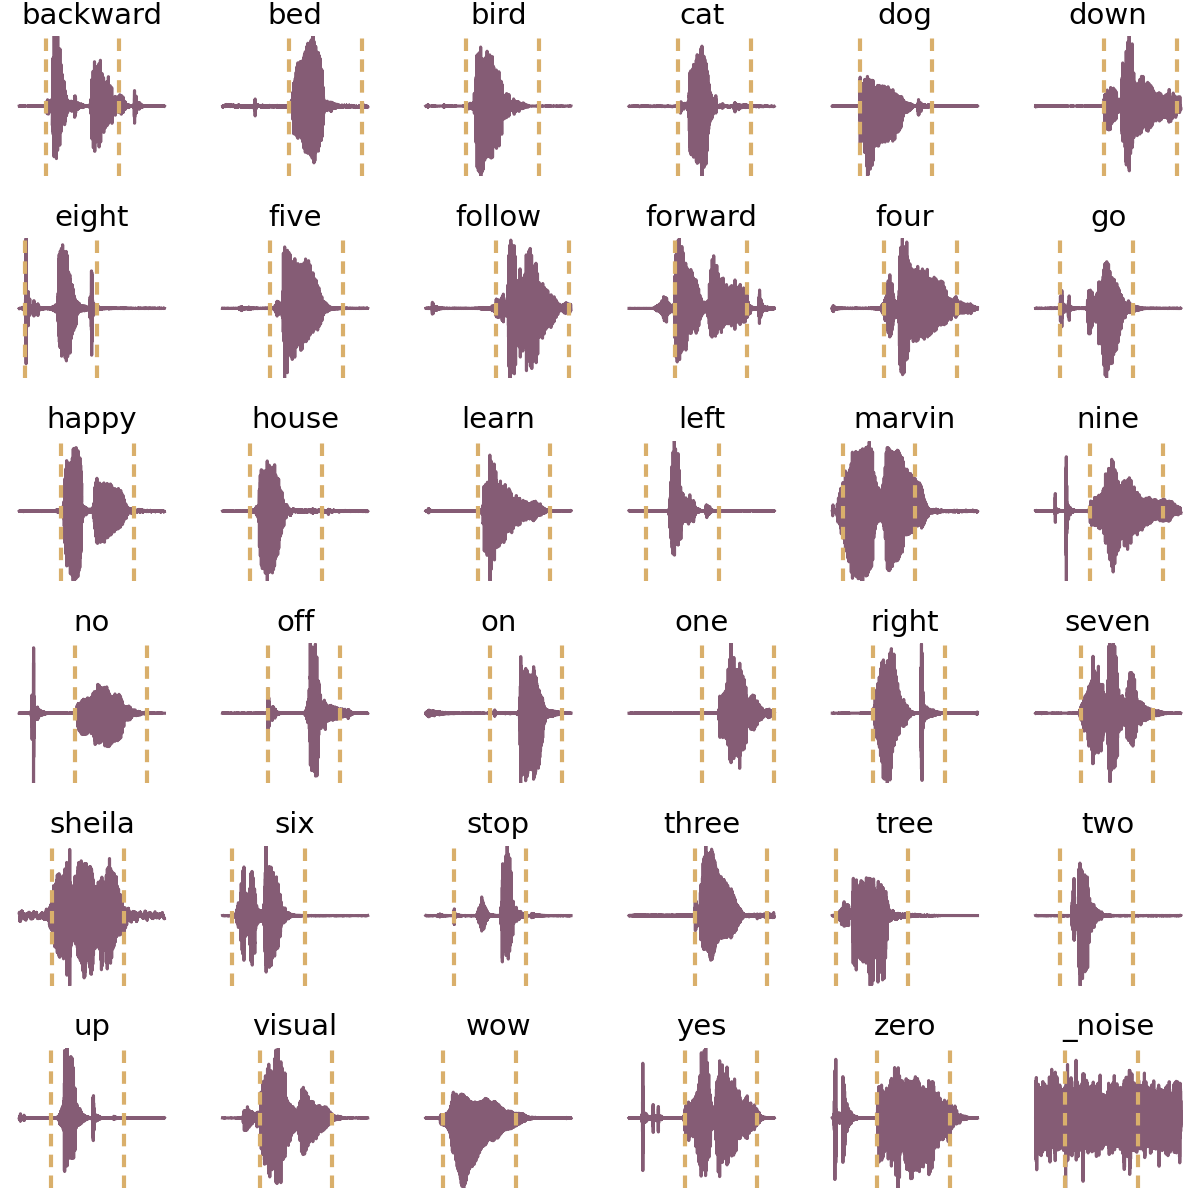
\includegraphics[width=0.9\textwidth]{../5_exp/figs/exp_dataset_speech_cmd_wav_grid.png} \end{figure}
    \end{column}
  \end{columns}
\end{frame}

\begin{frame}
  \frametitle{MFCC Extracted Dataset Examples}
  \vspace{-0.5cm}
  \begin{figure}[!ht]
    \centering
    \subfloat[left]{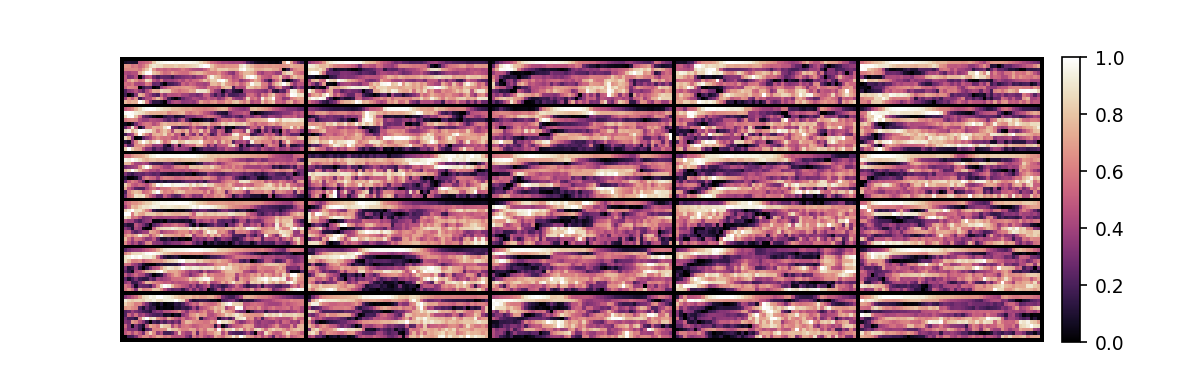
\includegraphics[width=0.8\textwidth]{../5_exp/figs/exp_dataset_speech_cmd_mfcc_left.png}}\\
    \vspace{-0.1cm}
    \subfloat[right]{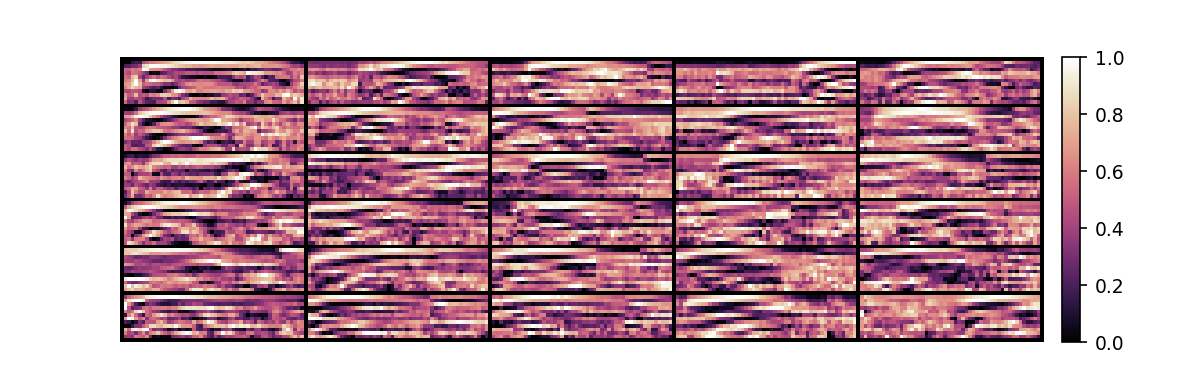
\includegraphics[width=0.8\textwidth]{../5_exp/figs/exp_dataset_speech_cmd_mfcc_right.png}}
  \end{figure}
\end{frame}

\begin{frame}
  \frametitle{My Dataset}
  \begin{itemize}
    \item vocabulary: \{\enquote{left}, \enquote{right}, \enquote{up}, \enquote{down}, \enquote{go}\}
    \item 5 examples per label
    \item used as additional test set
  \end{itemize}
  \vspace{-0.3cm}
  \begin{figure}[!ht]
    \centering
    \subfloat[audio]{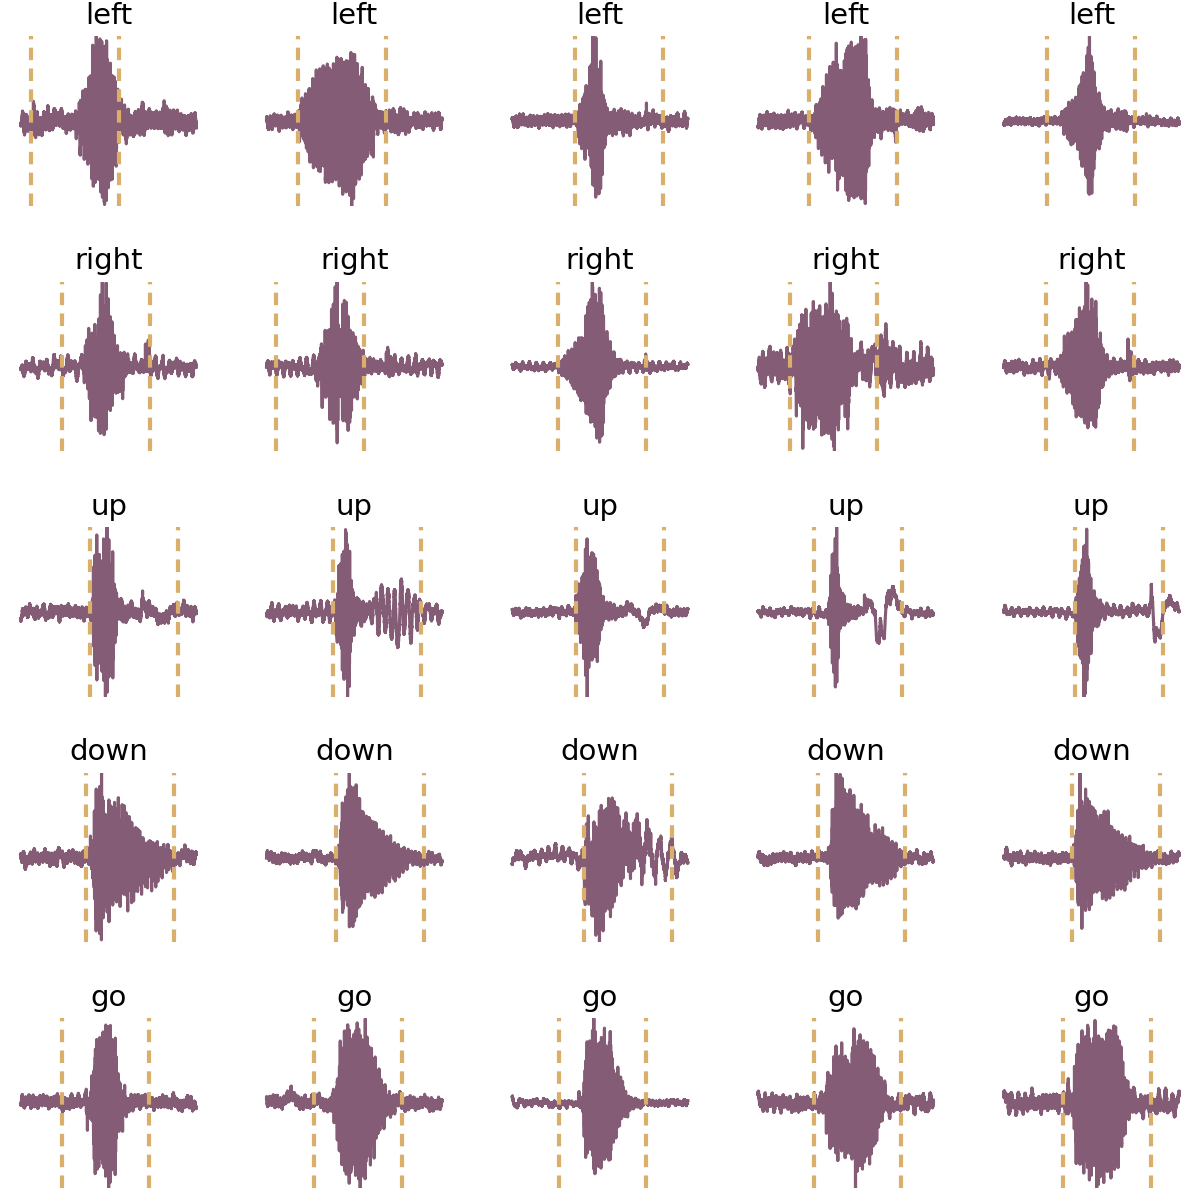
\includegraphics[width=0.29\textwidth]{../5_exp/figs/exp_dataset_my_wav_grid.png}}
    \subfloat[MFCC]{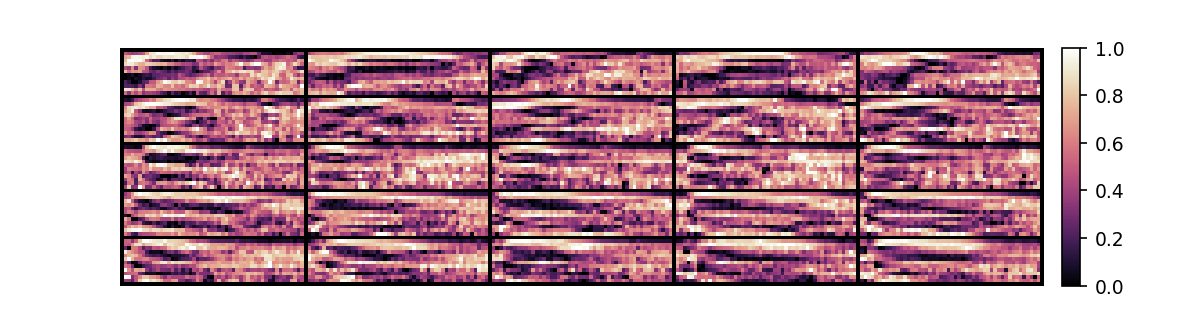
\includegraphics[width=0.69\textwidth]{../5_exp/figs/exp_dataset_my_mfcc.png}}
  \end{figure}
\end{frame}

\begin{frame}
  \frametitle{Feature Extraction Details for CNNs}
  \centering \vfill
  \begin{table}[ht!]
\scriptsize
\begin{center}
\begin{tabular}{ M{4cm}  M{1.5cm} M{1.5cm}}
\toprule
\textbf{Parameter} & \textbf{Value} & \textbf{Varying} \\
\midrule
Speech signal length & \SI{500}{\milli\second} & - \\
Analytic window size & \SI{25}{\milli\second} & -\\
Hop size & \SI{10}{\milli\second} & -\\
Window Function & Hanning & -\\
\midrule
Number of filter bands & 32 & -\\
Number of cepstral coefficients & 12 & yes\\
Delta features & no & yes \\
Double delta features & no & yes \\
Energy features & no 	& yes \\
Frame based normalization & yes & yes\\
\bottomrule
\label{tab:exp_details_params_feature}
\end{tabular}
\end{center}
\end{table}
\end{frame}

\begin{frame}
  \frametitle{Dataset Details}
  \begin{itemize}
    \item 500 examples per label for basic experiments
    \item 3500 examples per label for the final experiment
  \end{itemize}
  \begin{table}[ht!]
\scriptsize
\begin{center}
\begin{tabular}{ M{4cm}  M{5cm}}
\toprule
\textbf{Parameter} & \textbf{Value} \\
\midrule
Class dictionary with 12 labels (L12) & \{\enquote{left},  \enquote{right}, \enquote{up}, \enquote{down}, \enquote{go}, \enquote{stop}, \enquote{yes}, \enquote{no}, \enquote{on}, \enquote{off}, \enquote{\_mixed}, \enquote{\_noise}\}\\
\midrule
Number of examples per label & 500 or 3500 (whole dataset) \\ 
\bottomrule
\label{tab:exp_details_params_dataset}
\end{tabular}
\end{center}
\end{table}

\end{frame}

\begin{frame}
  \frametitle{Trainings Details for CNNs}
  \centering \vfill
  \begin{table}[ht!]
\scriptsize
\begin{center}
\begin{tabular}{ M{4cm}  M{1.5cm} M{1.5cm}}
\toprule
\textbf{Parameter} & \textbf{Value} & \textbf{Varying} \\
\midrule
Number of epochs & 2000 & yes\\
Batch size & 32 & -\\
\midrule
Optimizer & Adam & -\\
Learning rate & 0.0001 & -\\
Momentum & 0.9 & -\\
\bottomrule
\end{tabular}
\end{center}
\end{table}
\end{frame}

\begin{frame}
  \frametitle{Pre-Trainings Details with GANs}
  \centering \vfill
  \begin{table}[ht!]
\scriptsize
\begin{center}
\begin{tabular}{ M{4cm}  M{1.5cm} M{1.5cm}}
\toprule
\textbf{Parameter} & \textbf{Value} & \textbf{Varying} \\
\midrule
Number of epochs & 1000 & yes\\
Batch size & 32 & -\\
\midrule
Optimizer & Adam & -\\
Learning rate Generator & 0.0001 & -\\
Learning rate Discriminator & 0.0001 & -\\
Momentum Generator & 0.9 & -\\
Momentum Discriminator & 0.9 & -\\
\bottomrule
\end{tabular}
\end{center}
\end{table}
\end{frame}

\begin{frame}
  \frametitle{Experiment: Feature Selection Cepstral Coeff.}
  \begin{itemize}
    \item run on all three CNN models
    \item evaluation of
    \begin{itemize}
     \item amount of cepstral coeffs
     \item frame-based normalization
    \end{itemize}
    \item validation accuracy during training:
  \end{itemize}
  \vspace{-0.5cm}
  \begin{figure}[!ht]
    \centering
    \subfloat[conv-trad]{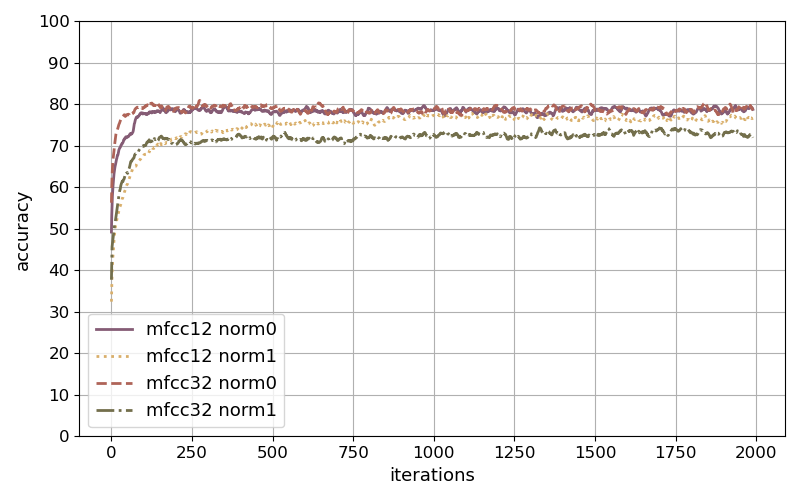
\includegraphics[width=0.48\textwidth]{../5_exp/figs/exp_fs_cepstral_acc_conv-trad.png}}
    \subfloat[conv-fstride]{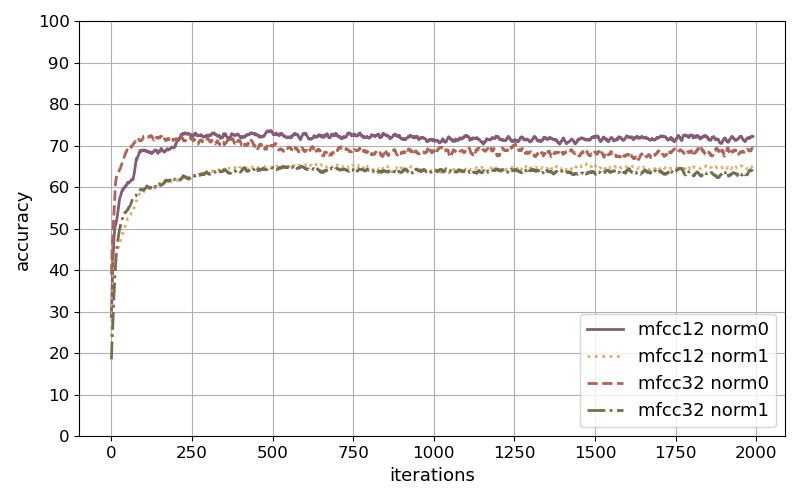
\includegraphics[width=0.48\textwidth]{../5_exp/figs/exp_fs_cepstral_acc_conv-fstride.png}}
  \end{figure}
\end{frame}

\begin{frame}
  \frametitle{Experiment: Feature Selection Cepstral Coeff.}
  \begin{figure}[!ht]
    \centering
    \subfloat[conv-jim]{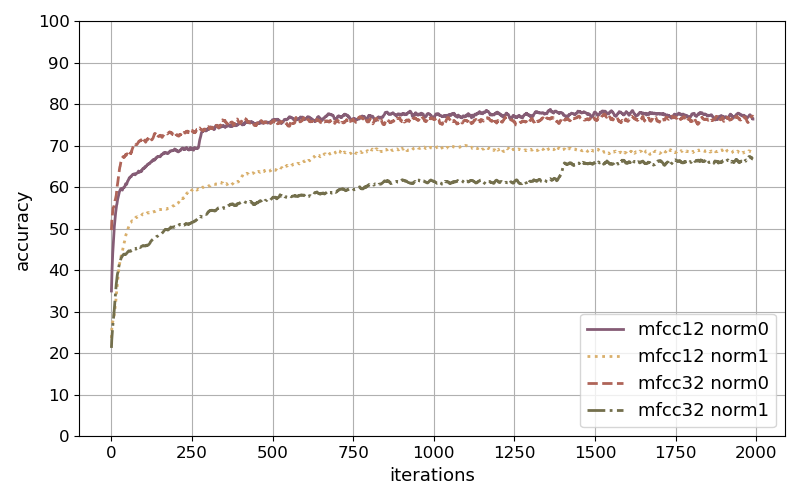
\includegraphics[width=0.75\textwidth]{../5_exp/figs/exp_fs_cepstral_acc_conv-jim.png}}
  \end{figure}
\end{frame}

\begin{frame}
  \frametitle{Experiment: Feature Selection Cepstral Coeff.}
  \begin{table}[ht!]
\scriptsize
\begin{center}
\begin{tabular}{ M{1.8cm}  M{1.5cm}  M{1cm}  M{2.2cm}  M{2.2cm} }
\toprule
\multirow{2}{1.8cm}{\centering\textbf{Model Name}} & \multirow{2}{1.5cm}{\centering\textbf{\# MFCC Coeffs.}} & \multirow{2}{*}{\centering\textbf{Norm.}} & \multicolumn{2}{c}{\textbf{Accuracy [\%]}}\\
&  &  & Test set & My dataset \\
\midrule
conv-trad & 12 & 0 & $80.57 \pm 0.34$ & $75.20 \pm 6.40$ \\
conv-trad & 12 & 1 & $76.17 \pm 1.02$ & $85.60 \pm 4.80$ \\
conv-trad & 32 & 0 & $79.77 \pm 1.56$ & $72.80 \pm 4.66$ \\
conv-trad & 32 & 1 & $74.63 \pm 1.13$ & $78.40 \pm 3.20$ \\
\midrule
conv-fstride & 12 & 0 & $72.03 \pm 1.94$ & $78.40 \pm 1.96$ \\
conv-fstride & 12 & 1 & $64.53 \pm 1.32$ & $72.00 \pm 2.53$ \\
conv-fstride & 32 & 0 & $70.73 \pm 1.42$ & $72.00 \pm 5.66$ \\
conv-fstride & 32 & 1 & $62.63 \pm 1.79$ & $69.60 \pm 4.80$ \\
\midrule
conv-jim & 12 & 0 & $78.70 \pm 1.38$ & $76.00 \pm 8.76$ \\
conv-jim & 12 & 1 & $72.90 \pm 1.85$ & $64.00 \pm 8.39$ \\
conv-jim & 32 & 0 & $76.40 \pm 3.22$ & $77.60 \pm 5.43$ \\
conv-jim & 32 & 1 & $65.83 \pm 1.29$ & $65.60 \pm 5.43$ \\
\bottomrule
\end{tabular}
\end{center}
\end{table}
\end{frame}

\begin{frame}
  \frametitle{Experiment: MFCC Enhancements}
  \begin{itemize}
    \item run on conv-jim model with frame-based normalization and 12 MFCC
    \item evaluation of
    \begin{itemize}
     \item different enhancements (c: cepstral, d: delta, dd: double delta, e: energy vector(s))
    \end{itemize}
    \item validation accuracy of best enhancement combination:
  \end{itemize}
  \vspace{-0.5cm}
  \begin{figure}[!ht]
    \centering
    \subfloat{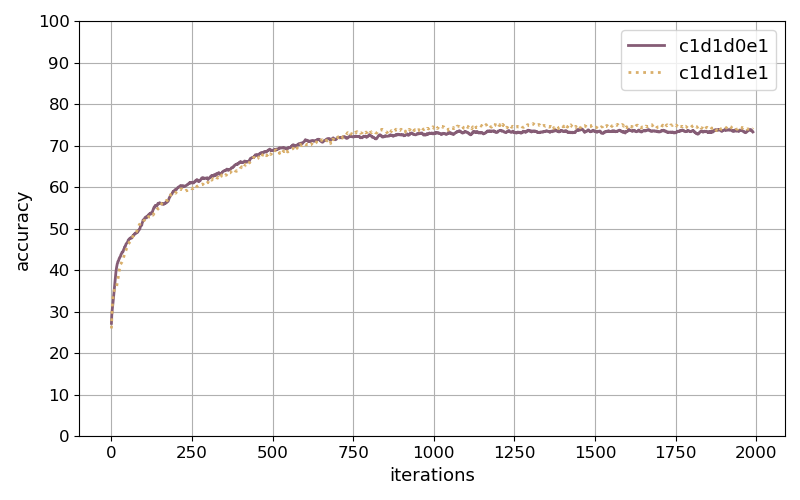
\includegraphics[width=0.48\textwidth]{../5_exp/figs/exp_fs_mfcc_acc_conv-jim.png}}
  \end{figure}
\end{frame}

\begin{frame}
  \frametitle{Experiment: MFCC Enhancements}
  \begin{table}[ht!]
\scriptsize
\begin{center}
\begin{tabular}{ M{0.75cm}  M{0.75cm}  M{0.75cm}  M{0.75cm}  M{2.5cm}  M{2.5cm} }
\toprule
\multicolumn{4}{c}{\textbf{Feature Selection}} & \multicolumn{2}{c}{\textbf{Accuracy [\%]}}\\
c & d & dd & e & Test set & My dataset\\
\midrule
0 & 0 & 1 & 0 & $37.40 \pm 2.17$ & $34.40 \pm 11.20$ \\
0 & 0 & 1 & 1 & $46.63 \pm 2.87$ & $36.80 \pm 7.76$ \\
0 & 1 & 0 & 0 & $58.57 \pm 2.06$ & $64.80 \pm 4.66$ \\
0 & 1 & 0 & 1 & $62.00 \pm 1.82$ & $75.20 \pm 11.14$ \\
0 & 1 & 1 & 0 & $59.03 \pm 1.77$ & $56.00 \pm 9.47$ \\
0 & 1 & 1 & 1 & $61.60 \pm 2.28$ & $62.40 \pm 6.97$ \\
1 & 0 & 0 & 0 & $72.00 \pm 1.46$ & $85.60 \pm 1.96$ \\
1 & 0 & 0 & 1 & $72.83 \pm 1.22$ & $80.00 \pm 4.38$ \\
1 & 0 & 1 & 0 & $70.63 \pm 2.13$ & $84.00 \pm 8.76$ \\
1 & 0 & 1 & 1 & $72.36 \pm 2.27$ & $80.00 \pm 4.38$ \\
1 & 1 & 0 & 0 & $72.80 \pm 2.90$ & $88.80 \pm 6.88$ \\
1 & 1 & 0 & 1 & $75.30 \pm 1.38$ & $92.00 \pm 2.53$ \\
1 & 1 & 1 & 0 & $73.43 \pm 2.05$ & $84.80 \pm 5.88$ \\
1 & 1 & 1 & 1 & $73.73 \pm 1.66$ & $83.20 \pm 6.88$ \\
\bottomrule
\end{tabular}
\end{center}
\end{table}
\end{frame}

\begin{frame}
  \frametitle{Experiment: Adversarial Label Train}
  \begin{itemize}
    \item run on conv-jim model with frame-based normalization and 12 MFCC
    \item evaluation of
    \begin{itemize}
     \item adversarial label train with different training epochs
     \item usage of either D or G filter weights
    \end{itemize}
    \item validation accuracy:
    \vspace{-0.5cm}
    \begin{figure}[!ht]
    \centering
    \subfloat{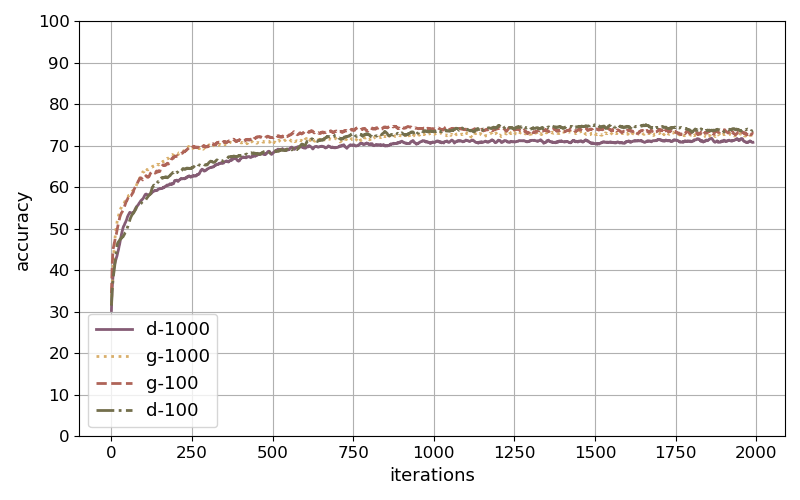
\includegraphics[width=0.48\textwidth]{../5_exp/figs/exp_adv_label_acc_conv-jim.png}}
    \end{figure}
  \end{itemize}
\end{frame}

\begin{frame}
  \frametitle{Experiment: Adversarial Label Train}
  \centering \vfill
  \begin{table}[ht!]
\scriptsize
\begin{center}
\begin{tabular}{ M{2cm}  M{2cm}  M{2.5cm}  M{2.5cm} }
\toprule
\multicolumn{2}{c}{\textbf{Adversarial}} & \multicolumn{2}{c}{\textbf{Accuracy [\%]}}\\
Epochs & Model & Test set & My dataset\\
\midrule
100 & G & $75.80 \pm 2.17$ & $85.60 \pm 4.08$ \\
100 & D & $73.57 \pm 1.59$ & $83.20 \pm 6.40$ \\
1000 & G & $74.83 \pm 2.15$ & $85.60 \pm 4.08$ \\
1000 & D & $73.36 \pm 0.86$ & $84.00 \pm 5.06$ \\
\bottomrule
\label{tab:exp_adv_label_l12}
\end{tabular}
\end{center}
\end{table}
\end{frame}

\begin{frame}
  \frametitle{Experiment: Wavenet}
  \begin{itemize}
    \item unfortunately poor classification results:
  \end{itemize}
  \vspace{-0.5cm}
  \begin{figure}[!ht]
    \centering
    \subfloat[validation accuracy]{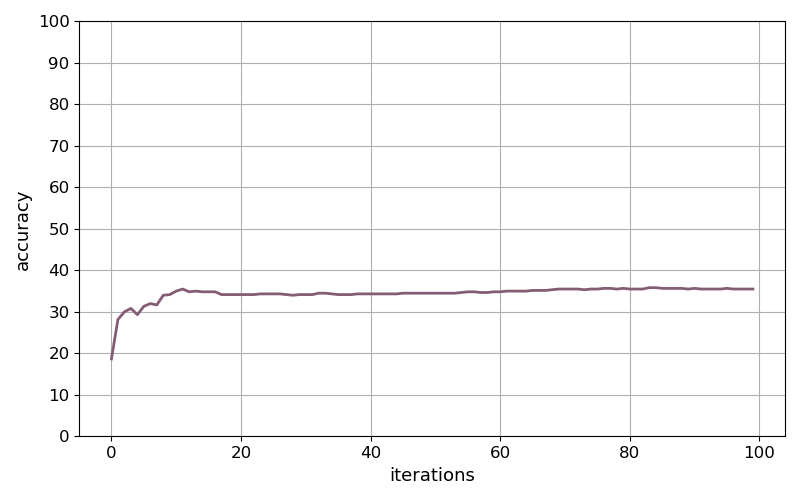
\includegraphics[width=0.45\textwidth]{../5_exp/figs/exp_wavenet_acc.png}}
    \subfloat[test confusion matrix]{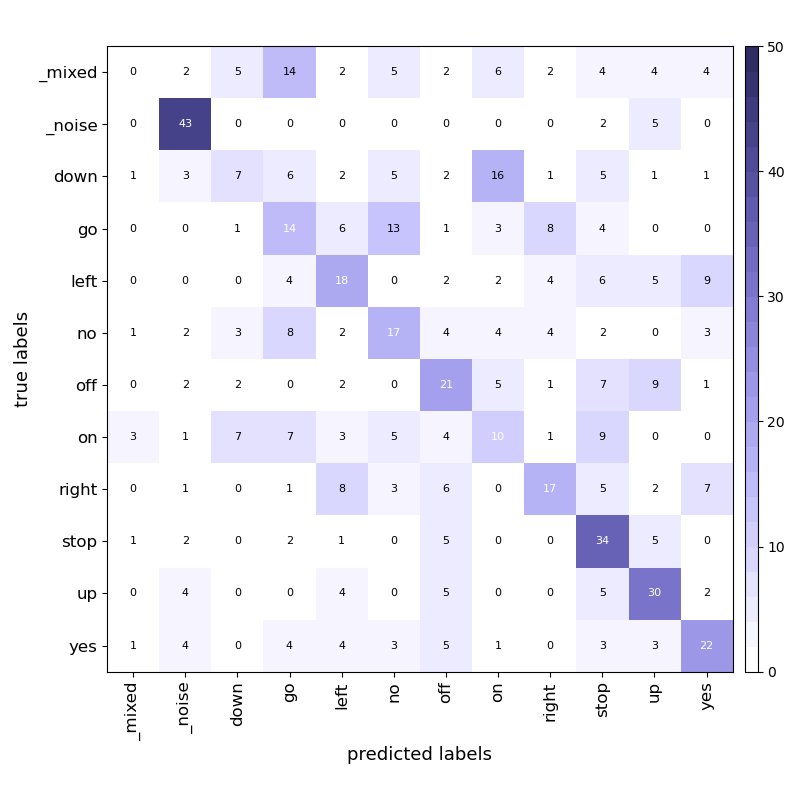
\includegraphics[width=0.45\textwidth]{../5_exp/figs/exp_wavenet_confusion_test.png}}
  \end{figure}
\end{frame}

\begin{frame}
  \frametitle{Experiment: Final}
  \begin{itemize}
    \item run on all CNN models the whole dataset
    \item evaluation of
    \begin{itemize}
     \item frame-based normalization
     \item adversarial label train
    \end{itemize}
    \item validation accuracy:
    \vspace{-0.5cm}
  \begin{figure}[!ht]
    \centering
    \subfloat[Norm.: 0]{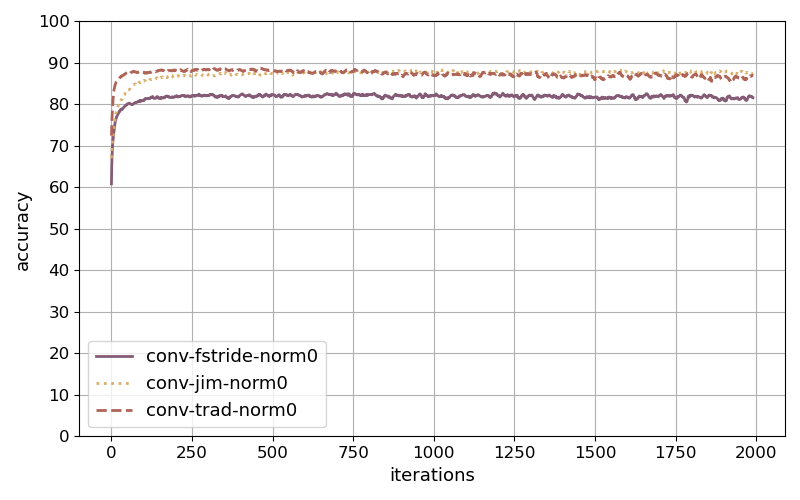
\includegraphics[width=0.48\textwidth]{../5_exp/figs/exp_final_acc_norm0.png}}
    \subfloat[Norm.: 1]{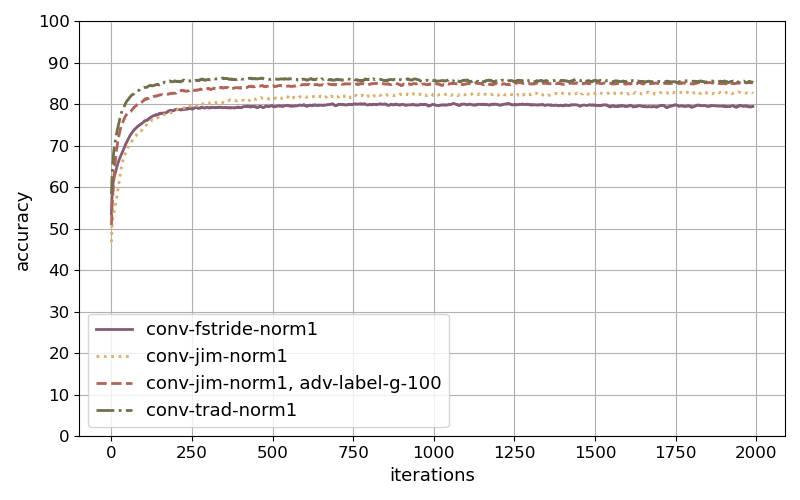
\includegraphics[width=0.48\textwidth]{../5_exp/figs/exp_final_acc_norm1.png}}
  \end{figure}
  \end{itemize}
\end{frame}

\begin{frame}
  \frametitle{Experiment: Final}
  \centering \vfill
  \begin{table}[ht!]
\scriptsize
\begin{center}
\begin{tabular}{ M{2cm}  M{1cm}  M{2cm}  M{1.75cm}  M{1.75cm} }
\toprule
\multirow{2}{*}{\centering\textbf{Model Name}} & \multirow{2}{*}{\centering\textbf{Norm.}} & \multirow{2}{*}{\centering\textbf{Pre-Train}} & \multicolumn{2}{c}{\textbf{Accuracy [\%]}}\\
& & & Test set & My dataset\\
\midrule
conv-trad & 0 & - & $84.52$ & $92.00$ \\
conv-fstride & 0 & - & $79.76$ & $80.00$ \\
conv-jim & 0 & - & $87.14$ & $88.00$ \\
\midrule
conv-trad & 1 & - & $83.79$ & $88.00$ \\
conv-fstride & 1 & - & $78.71$ & $92.00$ \\
conv-jim & 1 & - & $82.36$ & $88.00$ \\
\midrule
conv-jim & 1 & adv-label-100 & $84.62$ & $92.00$ \\
\bottomrule
\label{tab:exp_final_l12}
\end{tabular}
\end{center}
\end{table}
\end{frame}

\begin{frame}
  \frametitle{Experiment: Final}
  \begin{itemize}
      \item chosen model: conv-jim, frame-based normalized, adv-label-train
      \item confusion matrix on test set:
  \end{itemize}
  \begin{figure}[!ht] 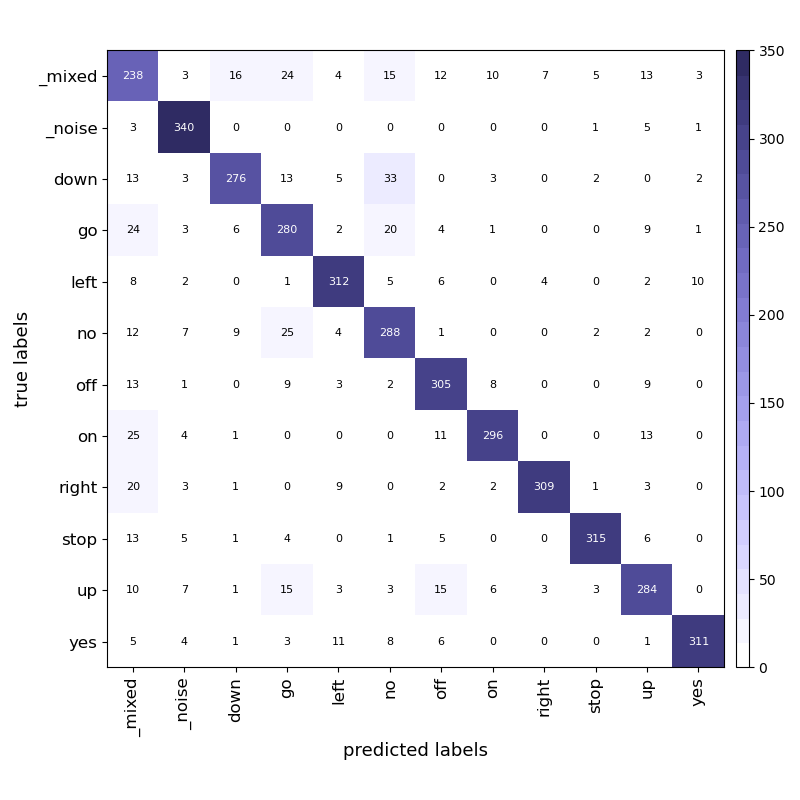
\includegraphics[width=0.45\textwidth]{../5_exp/figs/exp_final_confusion.png} \end{figure}
\end{frame}